% Transportation Research Board conference paper template
% version 1.1
% 
% David R. Pritchard, http://davidpritchard.org
%   1.0 - Mar. 2009
%   1.1 - Sep. 2011, fixes for captions

% PAGE LAYOUT
%------------------------------------------

% Custom paper settings...
\documentclass[titlepage,oneside,12pt]{article}

\oddsidemargin 0.0in
\topmargin -0.5in
\headheight 0.3in
\headsep 0.2in
\textwidth 6.5in
\textheight 9.0in
\setlength{\parindent}{0.5in}

\usepackage{hyperref}

% PAGE HEADER
%------------------------------------------
% Adjust the header text below (INSERT AUTHORS HERE)
\oddsidemargin 0.0in
\usepackage{lscape}
\usepackage[tiny,rm]{titlesec}
\usepackage{titling}
\usepackage{xcolor}
\newpagestyle{trbstyle}{
	\sethead{Apostolov and Oke}{}{\thepage}
}
\pagestyle{trbstyle}

% HEADINGS
%------------------------------------------
\titleformat{\section}{\bfseries}{}{0pt}{\uppercase}
\titlespacing*{\section}{0pt}{12pt}{*0}
\titleformat{\subsection}{\bfseries}{}{0pt}{}
\titlespacing*{\subsection}{0pt}{12pt}{*0}
\titleformat{\subsubsection}{\itshape}{}{0pt}{}
\titlespacing*{\subsubsection}{0pt}{12pt}{*0}

% LISTS
%------------------------------------------
% Adjust lists a little. Not quite perfectly fitting TRB style, but vaguely
% close at least.
%\usepackage{enumitem}
%\setlist[1]{labelindent=0.5in,leftmargin=*}
%\setlist[2]{labelindent=0in,leftmargin=*}

\usepackage{booktabs}
% CAPTIONS
%------------------------------------------
% Get the captions right. Authors must still be careful to use "Title Case"
% for table captions, and "Sentence case." for figure captions.
\usepackage{ccaption}
\usepackage{amsmath}
\makeatletter
\renewcommand{\fnum@figure}{\textbf{FIGURE~\thefigure} }
\renewcommand{\fnum@table}{\textbf{TABLE~\thetable} }
\makeatother
\captiontitlefont{\bfseries \boldmath}
\captiondelim{\;}
%\precaption{\boldmath}

% FONTS
%------------------------------------------
% Three options for fonts. I prefer Times for text and Computer Modern for
% math.

% Times for text, Computer Modern for math
\usepackage{times}
% Times for text and math
%\usepackage{pslatex}
% Times for text and math
%\usepackage{times,mathptmx} 

% Some pdf conversion tricks? Unsure.
\usepackage[T1]{fontenc}
\usepackage{textcomp}
\usepackage{bm}
\usepackage{makecell}
\usepackage{subfig}
\def\checkmark{\tikz\fill[scale=0.4](0,.35) -- (.25,0) -- (1,.7) -- (.25,.15) -- cycle;}

% CITATIONS
%------------------------------------------
% TRB uses an Author (num) citation style. I haven't found a way to make
% LaTeX/Bibtex do this automatically using the standard \trbcite macro, but
% this modified \trbcite macro does the trick.

% TODO: sort&compress option?
\usepackage[sort,numbers]{natbib}
\newcommand{\trbcite}[1]{({\it \citenum{#1}})}
\newcommand{\trbcitet}[1]{\citeauthor{#1} ({\it \citenum{#1}})}

\setcitestyle{round}

%% Cite Title
%\usepackage[style=authoryear,backend=biber,natbib,maxcitenames=2,doi=false,isbn=false,url=false,eprint=false]{biblatex}
%\addbibresource{bib/references.bib}

%\usepackage{hyperref}

% LINE NUMBERING
%------------------------------------------
% TRB likes line numbers on drafts to help reviewers refer to parts of the
% document. Comment out for final versions.
\usepackage{lineno}
\renewcommand\linenumberfont{\normalfont\small}
\linenumbers


% COUNTERS
%------------------------------------------
% TRB requires the total number of words, figures, and tables to be displayed on
% the title page. This is possible under the totcount package on CTAN.
\usepackage{totcount}
	\regtotcounter{table} 	%count tables
	\regtotcounter{figure} 	%count figures

\newcommand\wordcount{\immediate\write18{texcount -sum -1 \jobname.tex > 'count.txt'} \input{count.txt} }
  
% DOCUMENT START
%------------------------------------------
% Add any additional \usepackage declarations here.

\usepackage{graphicx}
\graphicspath{{./images/}}
 
\usepackage{rotating}
\usepackage{longtable}

%\usepackage{enumerate}
\usepackage{paralist}

%%%TIKZ
\usepackage{tikz}
\usepackage{pgfplots}
\usepackage{pgfplotstable}
\usepackage{pgfgantt}
\pgfplotsset{compat=newest}

\usetikzlibrary{arrows,shapes,positioning,shapes.geometric}
\usetikzlibrary{decorations.markings}
\usetikzlibrary{shadows,automata}
\usetikzlibrary{patterns}
\usetikzlibrary{trees,mindmap,backgrounds}
%\usetikzlibrary{circuits.ee.IEC}
\usetikzlibrary{decorations.text}
% For Sagnac Picture
\usetikzlibrary{%
    decorations.pathreplacing,%
    decorations.pathmorphing%
}
\tikzset{no shadows/.style={general shadow/.style=}}
%
%\usepackage{paralist}

%%% FORMAT PYTHON CODE
\usepackage{listings}
% Default fixed font does not support bold face
\DeclareFixedFont{\ttb}{T1}{txtt}{bx}{n}{8} % for bold
\DeclareFixedFont{\ttm}{T1}{txtt}{m}{n}{8}  % for normal

% Custom colors
\usepackage{color}
\definecolor{deepblue}{rgb}{0,0,0.5}
\definecolor{deepred}{rgb}{0.6,0,0}
\definecolor{deepgreen}{rgb}{0,0.5,0}

\newcommand{\osn}{\oldstylenums}
\newcommand{\dg}{^{\circ}}
\newcommand{\lt}{\left}
\newcommand{\rt}{\right}
\newcommand{\pt}{\phantom}
\newcommand{\tf}{\therefore}
\newcommand{\?}{\stackrel{?}{=}}
\newcommand{\fr}{\frac}
\newcommand{\dfr}{\dfrac}
\newcommand{\ul}{\underline}
\newcommand{\tn}{\tabularnewline}
\newcommand{\nl}{\newline}
\newcommand\relph[1]{\mathrel{\phantom{#1}}}
\newcommand{\cm}{\checkmark}
\newcommand{\ol}{\overline}
\newcommand{\rd}{\color{red}}
\newcommand{\bl}{\color{blue}}
\newcommand{\pl}{\color{purple}}
\newcommand{\og}{\color{orange!90!black}}
\newcommand{\gr}{\color{green!40!black}}
\newcommand{\nin}{\noindent}
\newcommand{\la}{\lambda}
\renewcommand{\th}{\theta}
\newcommand{\al}{\alpha}
\newcommand{\G}{\Gamma}
\newcommand*\circled[1]{\tikz[baseline=(char.base)]{
            \node[shape=circle,draw,thick,inner sep=1pt] (char) {\small #1};}}

\newcommand{\bc}{\begin{compactenum}[\quad--]}
\newcommand{\ec}{\end{compactenum}}

\newcommand{\p}{\partial}
\newcommand{\pd}[2]{\frac{\partial{#1}}{\partial{#2}}}
\newcommand{\dpd}[2]{\dfrac{\partial{#1}}{\partial{#2}}}
\newcommand{\pdd}[2]{\frac{\partial^2{#1}}{\partial{#2}^2}}

\begin{document}
\renewcommand{\refname}{\uppercase{References}}
% \raggedright

\begin{titlepage}
\begin{flushleft}

% Title
{\LARGE \bfseries Modeling the impacts of interventions and mobility patterns on COVID-19 country outcomes}\\[1cm]

%%%%%%%%%%%%%%%%%%%%%%%%%%%%%%
%%% Provisional author list; to be finalized once draft is ready.
%%%%%%%%%%%%%%%%%%%%%%%%%%%%%%5

 \textbf{Atanas Apostolov\textsuperscript{1}} \\
 Email: @; Phone:   \\[0.5cm]

 \textbf{Jimi B.\ Oke\textsuperscript{1}} \\
 %\textit{Corresponding Author} \\
 Email: @; Phone:  \\[0.5 cm]

% \textbf{Author 3 \textsuperscript{1}} \\
% Email: @ ; Phone: \\[0.5 cm]
 
 
\textbf{\textsuperscript{1} Department of Civil and Environmental Engineering, University of Massachusetts Amherst, MA 01003, United States} \\[0.3 cm]
%\textbf{\textsuperscript{2} Department of Civil and Environmental Engineering, University of Massachusetts Amherst, MA 01003, United States} \\[0.3 cm]


\wordcount words + \total{table} tables %+ \total{figure} figures

\today

\end{flushleft}
\end{titlepage}

%% This generates the title page from the information given above.
\thispagestyle{empty}
%\maketitle

\newpage

\thispagestyle{empty}
 

\section{Abstract}
In this paper we examine the effects of COVID-19 on mobility, segmented by transportation type, as well as social activity such as retail and recreation, workplaces and residential. We use time series data for approximately sixty countries on five continents to discover a statistically significant relationship between mobility and new COVID-19 cases. We hope that the findings of this paper will guide policymakers to adopt an appropriate set of measures in order to reduce the infection rate and ease social restrictions in a safe manner.

\section{Introduction}
COVID-19 has had a severe impact on mobility and social activities since initial reports of the disease emerged in late 2019.
By May 2020 most countries had implemented social distancing measures and imposed strict travel restrictions to curtail the spread of the virus
both within their borders and internationally.
According to \trbcite{bonaccorsi2020economic}, the international spread of the disease can be partially explained by risk perception,
mobility behavior and social media influences using a global vector autoregression (GVAR) modeling framework\cite{dees2007exploring}.
%Milani concludes that most countries learn from each other's social distancing response which can be partially explained by social networks.  
\trbcite{zhang2020pathways} confirm that human mobility is key to understanding the transmission pathways.
Using a mobility dataset of over 500,000 flights and over 100 million passengers,
the authors develop a dynamic network model using time-dependent border restrictions as exogenous variables.
\trbcite{mckenzie2020country} studied the patterns in 6 activity responses across 108 countries but this was an exploratory effort in comparison with government policies and it included no modeling attempt to explain COVID-19 outcomes.

Beyond these global studies, several city and country-specific simulations and models have been estimated to explain how activities, mobility (particularly transit) impact COVID-19 outcomes.
\trbcite{kumar2020activitybaseda} used an activity-based epidemiological framework to study how COVID-19 is propagated across various daily activities in car-dependent cities typically found in the US and Canada.
They quantified the effect of the transit network on COVID-19 spread and demonstrated the importance of work and home activities in the early and latter stages of the epidemic.
\trbcite{badr2020association} developed a generalized linear model to explain COVID-19 growth based on overall mobility changes at the county level in the US. Inter-county movements were factored in but impacts by mode or activity were not analyzed.
Given China's and then  Italy's prominence in the earlier stages of the pandemic, several studies have examined their mobility patterns \trbcite{
  kraemer2020effect,bonaccorsi2020economic,pepe2020covid19,carteni2020how}.
While these have been important for country-wide epidemiological studies, they have not provided knowledge on activity-based impacts.

Therefore, there remains an urgent need to understand the interdependcies between COVID-19 outcomes and human mobility and activity patterns.
Statistically significant models can yield insights to enable policymakers contain and recover from the ongoing pandemic.
Furthermore, these models can guide future decisions in containing the spread of future epidemics.
In this paper, we conduct a global scale country-level analysis of COVID-19 infections,  mobility and activity patterns.
First, we cluster the countries to discover patterns in mobility and activity changes.
Second, we estimate cluster-represenative models using the vector autoregression (VAR) framework, allowing for time lags across all endogenous variables, and thus including dynamic interdependencies among them.
These models explain which activities impact COVID-19 outcomes and vice versa, providing potential pathways for understanding behavioral responses to the spread of the pandemic and a greater understanding of the disparities and similarities across nationwide outcomes.

%By assigning a value of zero or one to international mobility restrictions, Zhang et al discover a direct relationship between the transmission rates and the coefficients in the estimation outcome, i.e. positive coefficients indicate effectiveness. 

% \trbcite{forecasting} shed light on forecasting with Bayesian Global Vector Autoregressive Model. This statistical approach pertains to the impacts of mobility on COVID-19 due to its counterfactual nature; instead of treating observations in isolation B-GVAR accommodates variable interdependence and produces more robust forecasts. Country-specific models can be converted to a system of equations where all endogenous variables are stacked. Although taking into account international linkages improves the forecast, the optimal lag for each country still needs to be estimated and tested for stationarity 




\section{Data}
We use transportation data provided by Apple \footnote{\url{https://www.apple.com/covid19/mobility}} along with Community Mobility Reports compiled by Google\footnote{\url{https://www.google.com/covid19/mobility/}}. %The data is publicly available at:
The new confirmed cases global data set is provided by the Johns Hopkins University COVID-19 Data initiative\footnote{\url{https://github.com/CSSEGISandData/COVID-19}}.
Apple's dataset focuses on transportation types (walking, driving, transit) whereas Google tracks movement trends by region and segments them into categories such as residential, workplace and transit. Our integrated data set captures changes in requests for directions from January 22 to July 14 as well as aggregated location data for a variety of categorized places. The data shows us the change in visitors from February 15 to July 12 compared to a baseline of days (January 3 - February 6, 2020). By tracking user requests of their Maps application, Apple contributes a snapshot of incidental trips as opposed to actual foot traffic which is the approach taken by Google for their Community Mobility Reports. 

\begin{table}[h!]\small
\begin{tabular}{ll}\toprule
\bf Source                         & \bf Overview                                                                              \\\midrule
Johns Hopkins University          & Time series summary globally.                                                               \\
Apple Maps                        & Compared to a baseline volume on January 13th, 2020.                                          \\
  Google Community Mobility Reports & Compared to a baseline day \\
  & (median value over period from Jan 3 to Feb 6, 2020)\\\bottomrule
\end{tabular}
\end{table}

\begin{table}[]
  \centering
    % \begin{tabular}{l l l l}\toprule
    %     \bf Variable & \bf Date & \bf Coverage & \bf Description  \\ 
    %      & & & \\\bottomrule
    % \end{tabular}

\caption{Summary of variables}
\label{tab:my_label}

  \small
\begin{tabular}{ll}\toprule
\textbf{Variable}                                         & \textbf{Description}                                    \\\midrule
confirmed\_cases                                         & Newly confirmed cases of COVID-19              \\
driving                                                  & Requests for driving directions in Apple Maps.    \\
walking                                                  & Requests for walking directions in Apple Maps   \\
transit                                                  & Requests for transit directions in Apple Maps   \\
retail\_and\_recreation\_percent\_change\_from\_baseline & Retail and recreation movement trends.            \\
grocery\_and\_pharmacy\_percent\_change\_from\_baseline  & Grocery and pharmacy movement trends.             \\
parks\_percent\_change\_from\_baseline                   & Parks movement trends.                           \\
transit\_stations\_percent\_change\_from\_baseline       & Transit stations movement trends.                \\
workplaces\_percent\_change\_from\_baseline              & Workplaces movement trends.                      \\
residential\_percent\_change\_from\_baseline             & Retail and recreation movement trends.          \\\bottomrule
\end{tabular}
\end{table}




The integrated dataset is publicly available on Github.\footnote{\url{https://github.com/narslab/covid-analysis/tree/master/mobility}}

\begin{figure}[h!]
    \centering
    %\includegraphics[width=.6\textwidth]{mobility_graph.png}
    \caption{Caption}
    \label{fig:my_label}
\end{figure}

%\href{https://github.com/narslab/live-dashboard}{Dashboard}
%\url{https://github.com/narslab/live-dashboard}

\section{Methods}

\subsection{Dynamic time warping}
The dynamic time warping (DTW) algorithm \trbcite{giorgino2009computing} computes the optimal distance between pairwise time series.
Any hierarchical clustering procedure requires a dissimilarity matrix as an input, which DTW provides.
First, we compute the Euclidean distance matrix for each country across the dimensions of the endogenous variables.
Second, we apply DTW to find the optimal matching between the countries based on their pairwise distance matrices across the dimensions observed.
The symmetric dissimilarity matrix is then used an input to the clustering algorithm.


\subsection{Clustering}
We use the Ward method \trbcite{murtagh2014ward}, which is a hierarchical agglomerative clustering (HAC) approach to group the countries.
The dendogram is shown in \autoref{fig:dend}.



% We use a Global Vector AutoRegression (GVAR) modeling framework \cite{dees2007exploring} (Carteni et al
% 2020).
% Given country $i$ with $k_{i}$ endogenous variables $x_{i,t}$, the model is specified as
% \begin{equation}
%   \label{eq:1}
%   x_{i,t} = \sum_{l=1}^{p_{i}}\Phi_{il}x_{i,t-l} + \Lambda_{i0}x_{i,t}^{*} + \sum_{l=1}^{q_{i}} \Lambda_{il}x_{i,t-l}^{*} + \varepsilon_{i,t}
% \end{equation}
% where $i= 1, 2, \ldots, N$. The matrix $\Phi_{il}$ is the matrix of coefficients of size $k_{i}\times k_{i}$, while the matrix $\Lambda_{i0}$ and $\Lambda_{il}$ are $k_{i}\times k_{i}^{*}$ matrices, where $k_{i}^{*}$ is the number of foreign variables.

% We can stack the domestic and foreign variables as:
% \begin{equation}
%   \label{eq:2}
%   z_{i,t} = [x_{i,t}', x_{i,t}^{*'}]'
% \end{equation}
% and then rewrite the model as :
% \begin{equation}
%   \label{eq:3}
%   A_{i0}z_{i,t} = \sum_{i=1}^{p} A_{il}z_{i,t-l} + \varepsilon_{i,t}
% \end{equation}
% where
% \begin{align}
%   \label{eq:4}
%   A_{i0} &= (I_{k_{i}} - \Lambda_{i0}) \\
%   A_{il} &= \Phi_{il}\Lambda_{il}
% \end{align}
% for $l = 1,\ldots, p$.

% The weakly exogenous (foreign) variables are given by
% \begin{equation}
%   \label{eq:5}
%   x_{i,t}^{*} = \sum_{j\ne i}w_{ij} x_{j,t}
% \end{equation}
% where $w_{ij}$ are the cross-country weights.




\subsection{Vector autoregression model}
The vector autoregression (VAR) model is given by:
\begin{equation}
  \label{eq:6}
  y_{it} = A_{0i}(t) + A_{i}(\ell)Y_{t-1} + \varepsilon_{it}
\end{equation}
where $y_{it}$ is a $k\times 1$ vector of endogenous variables for country $i\in\{1,\ldots,N\}$ at time $t\in \{1,\ldots, T\}$,
$A_{0i}(t)$ captures the deterministic components (fixed effects) of country $i$
$A(\ell)$ is a polynomial in the lag operator and $\varepsilon_{it}\sim iid(0,\Sigma_{\varepsilon})$ are random disturbances

This framework allows for specification of both dynamic and static interdependencies
among the endogenous variables, as well as cross-sectional heterogeneities.

In this case, the domestic variables are as follows (growth rates computed as difference of logs):
% \begin{itemize}
% \item COVID cases $y_{1}$
% \item driving $y_{2}$
% \item transit $y_{3}$
% \item walking $y_{4}$
% \item retail and recreation $y_{5}$
% \item grocery and pharmacy $y_{6}$
% \item parks $y_{7}$
% \item transit stations $y_{8}$
% \item work $y_{9}$
% \item home $y_{10}$
% \end{itemize}


\section{Results and Discussion}



\begin{figure}[h!]
  %\centering
  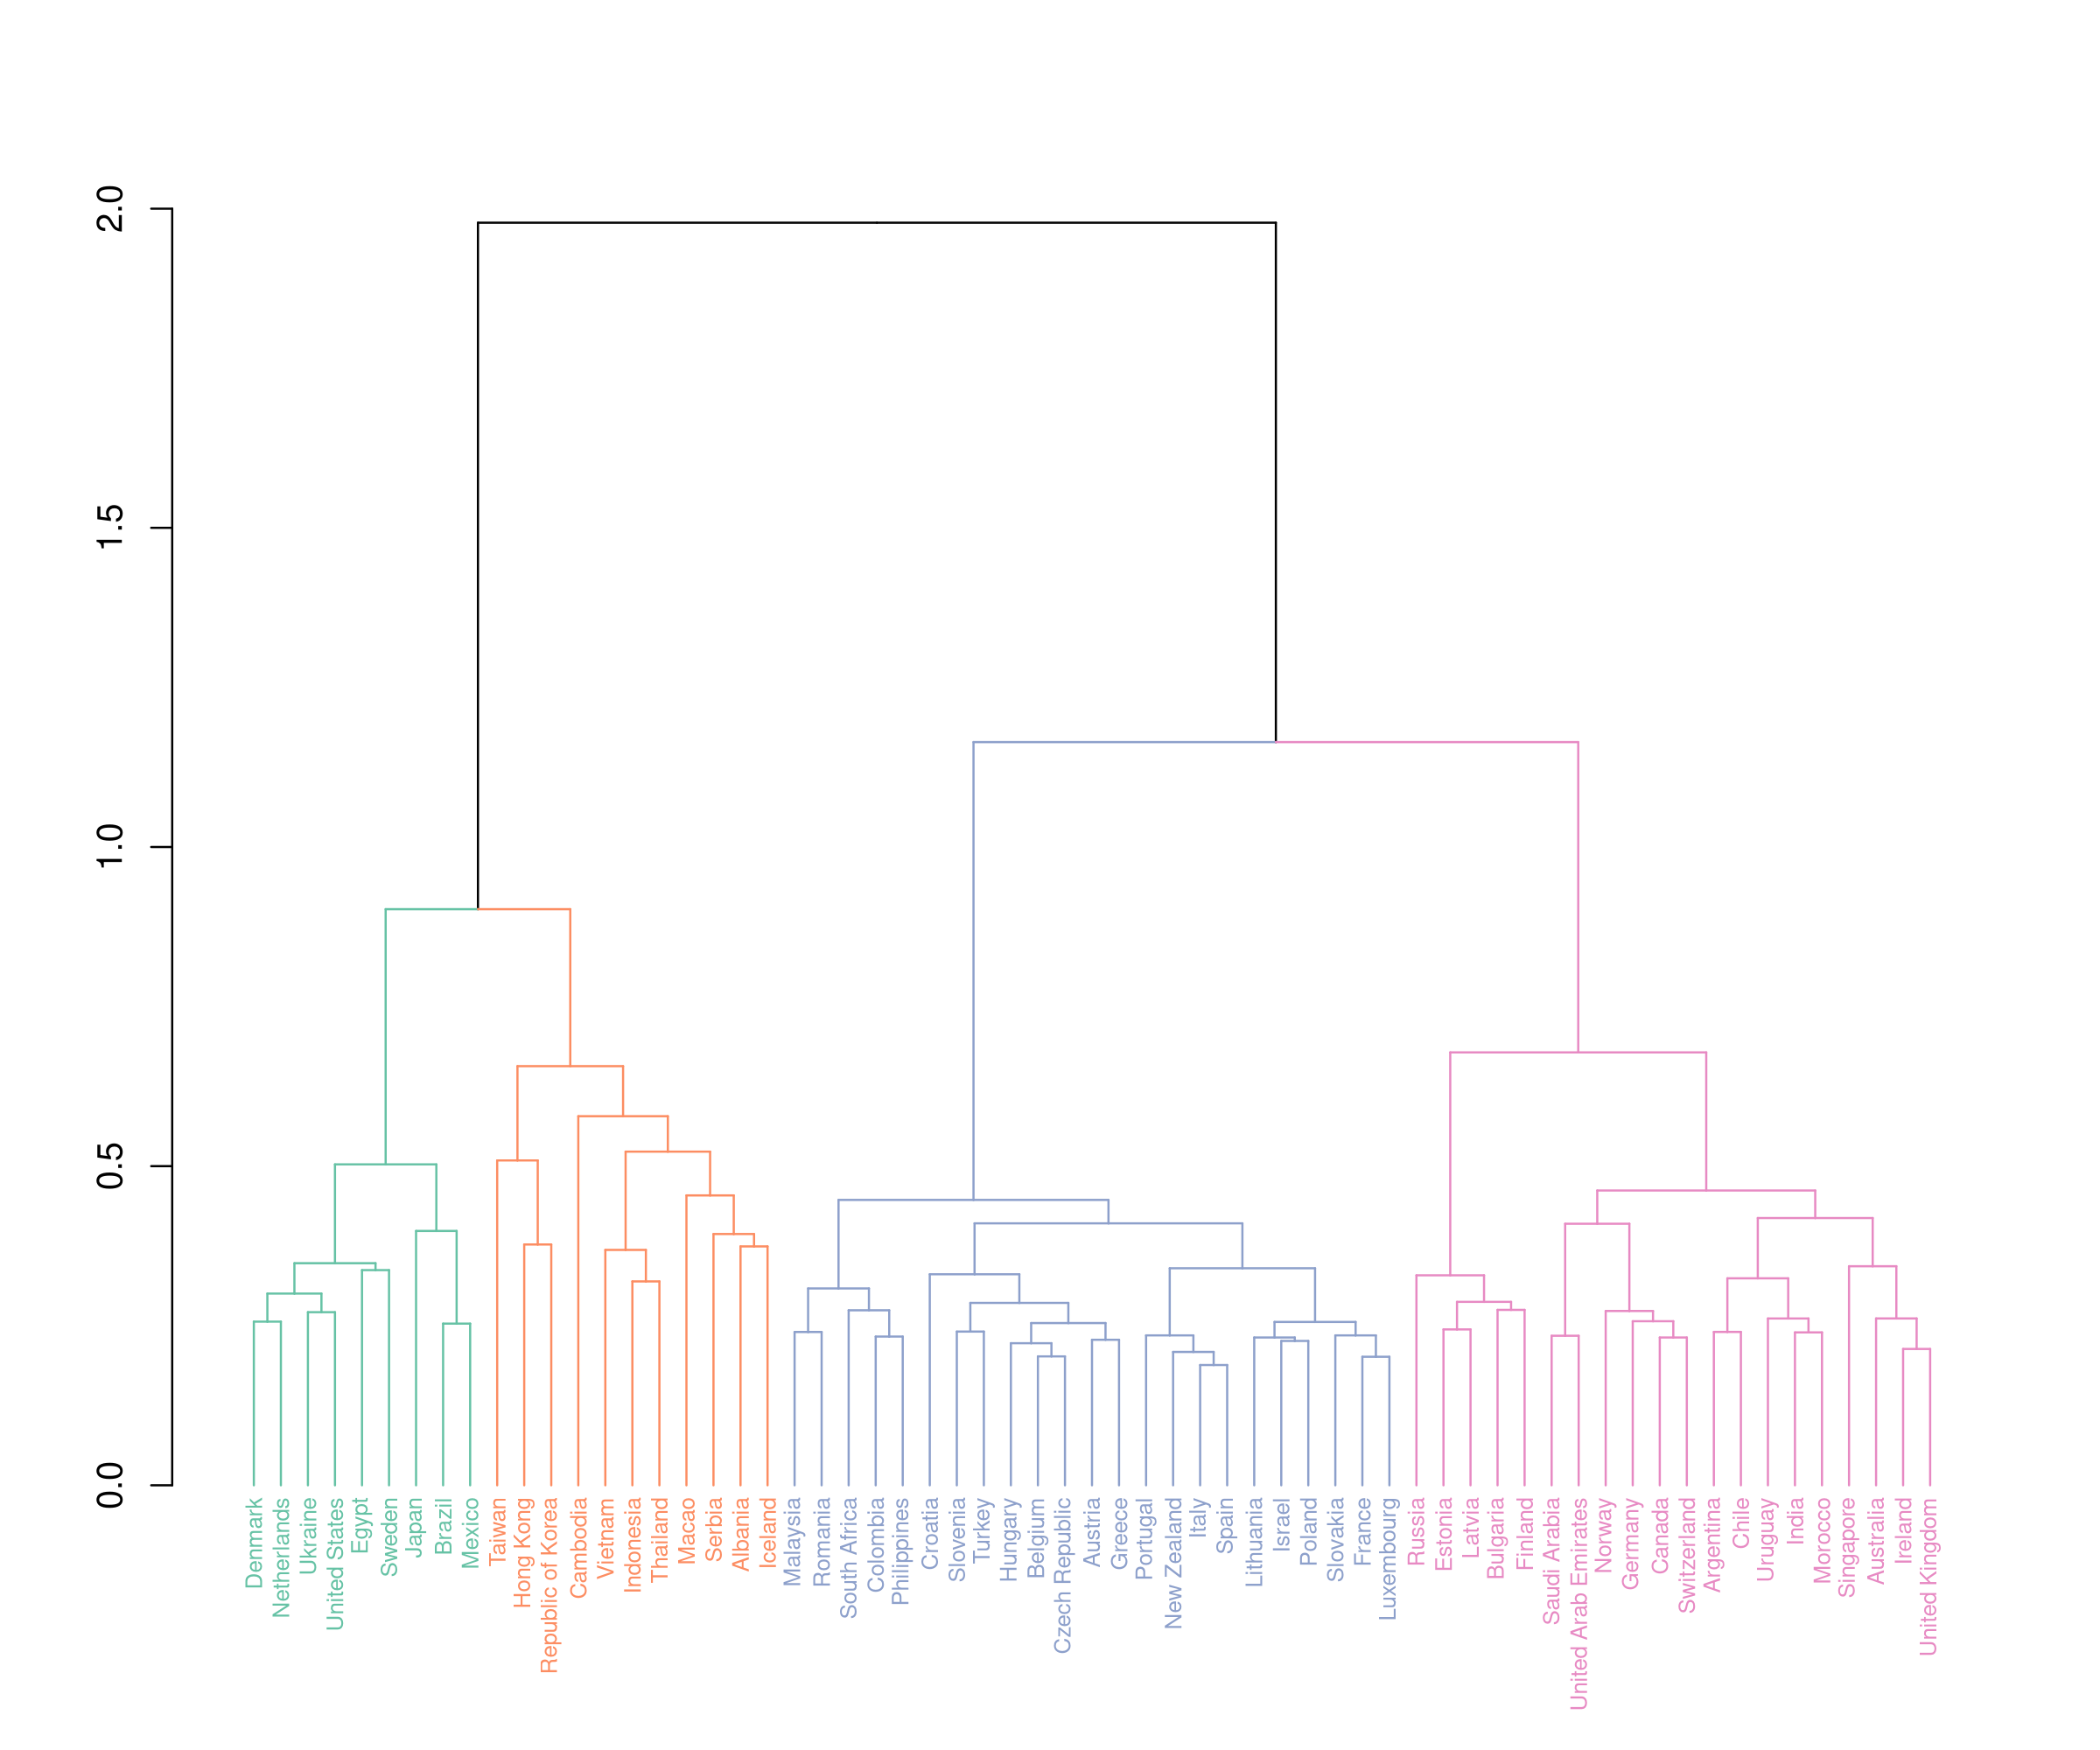
\includegraphics[width=\textwidth,trim={0cm 0 1.9cm 7cm},clip]{dendrogram}
  \caption{Dendrogram indicating four clusters of countries based on nine mobility and activity indicators}
  \label{fig:dend}
\end{figure}



\begin{figure}[h!]
  \centering
  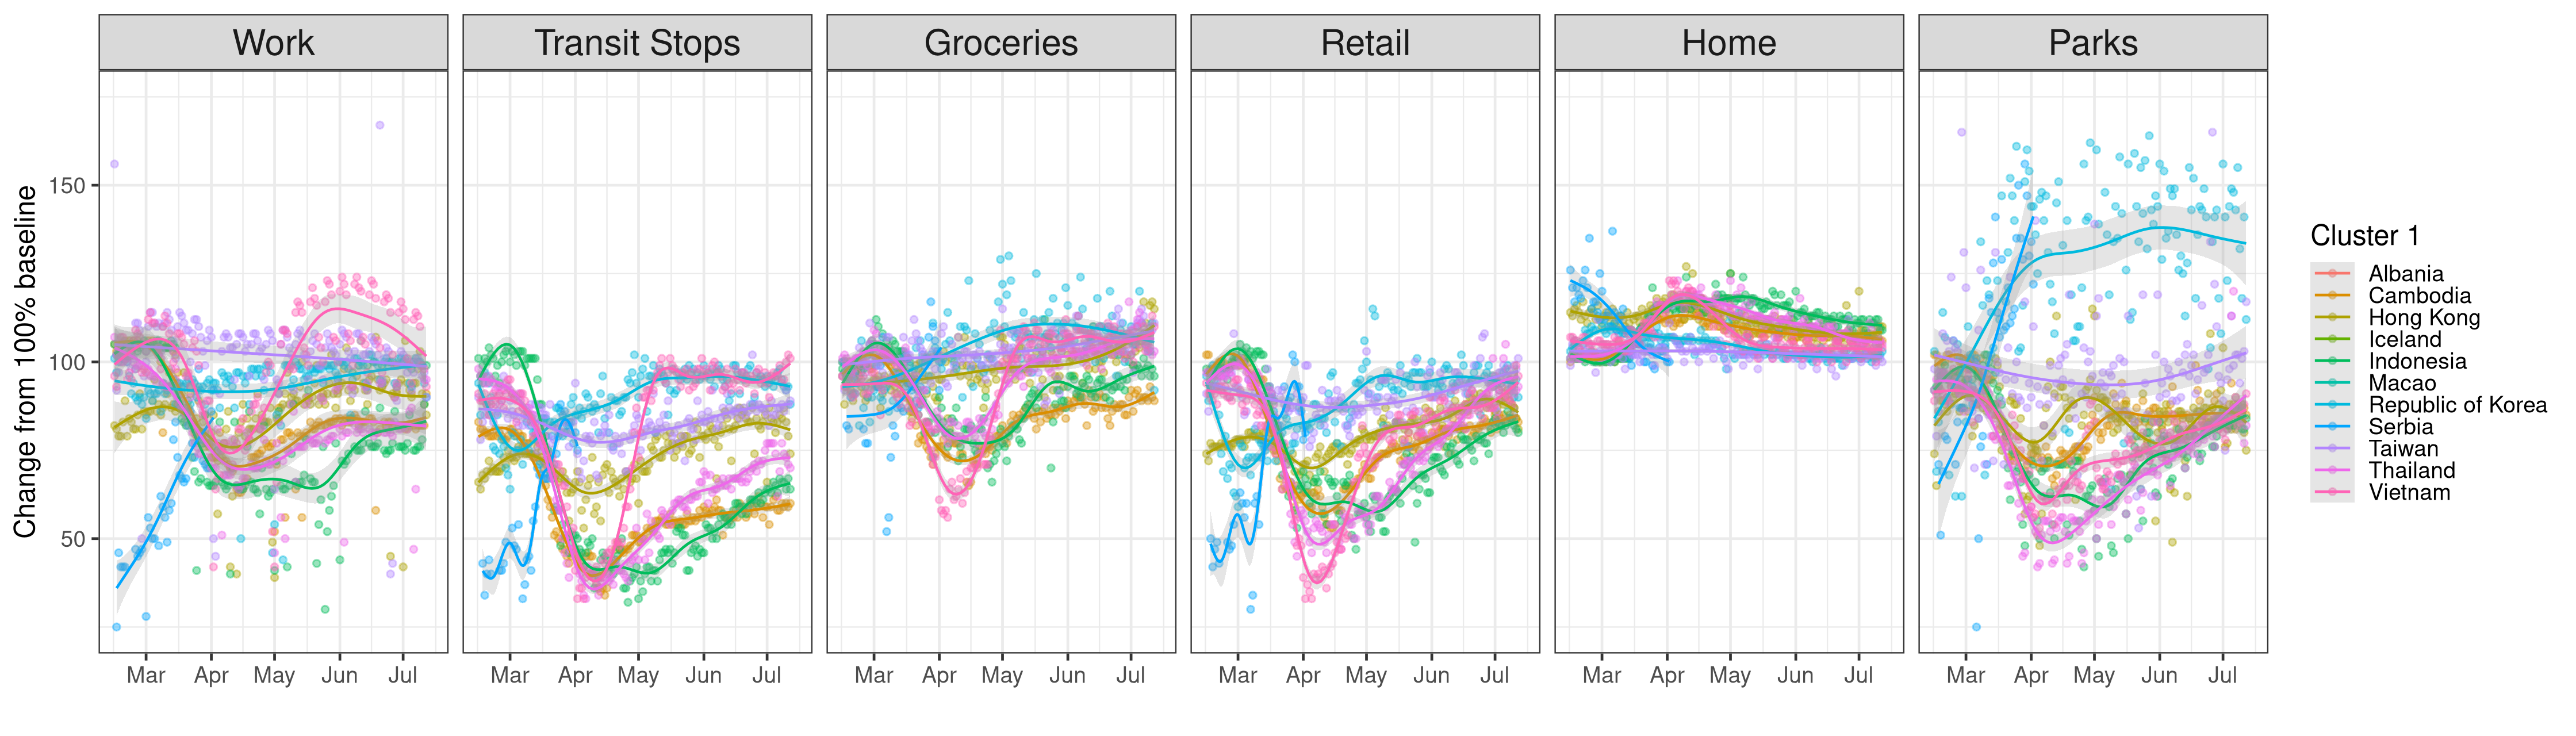
\includegraphics[width=\textwidth]{c1-activity}
  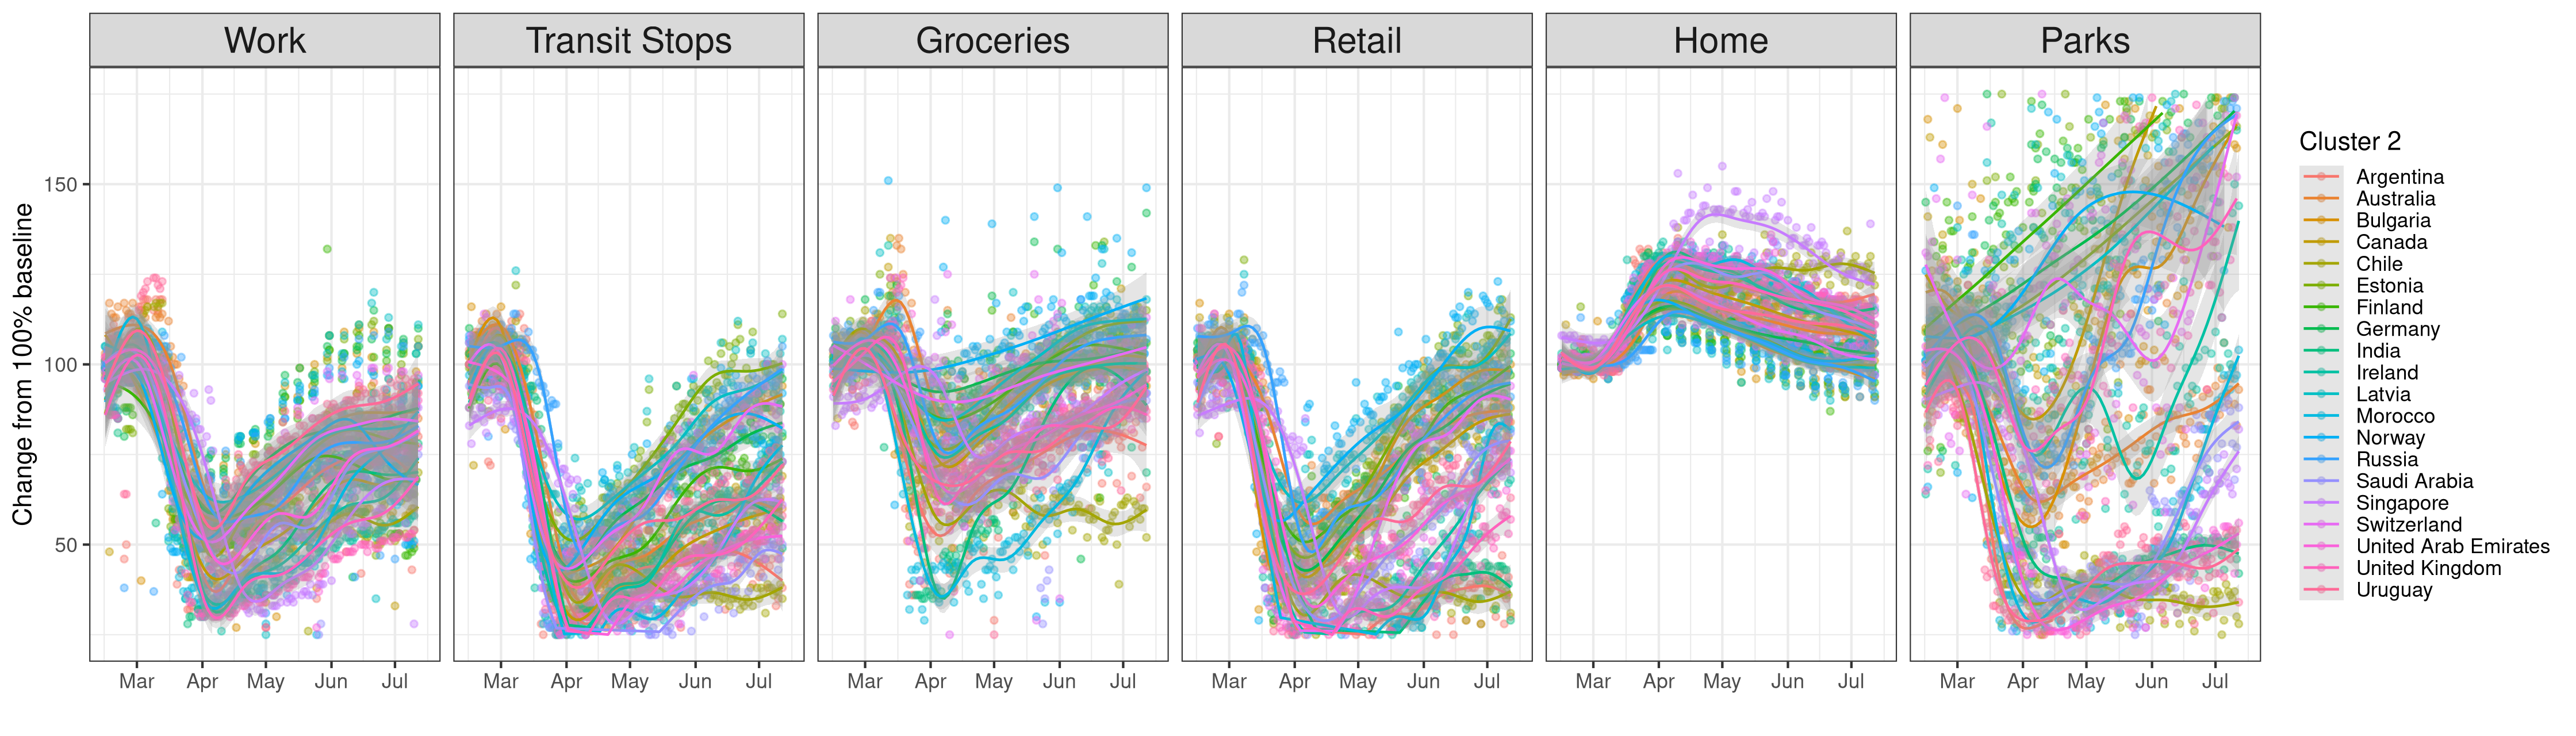
\includegraphics[width=\textwidth]{c2-activity}
  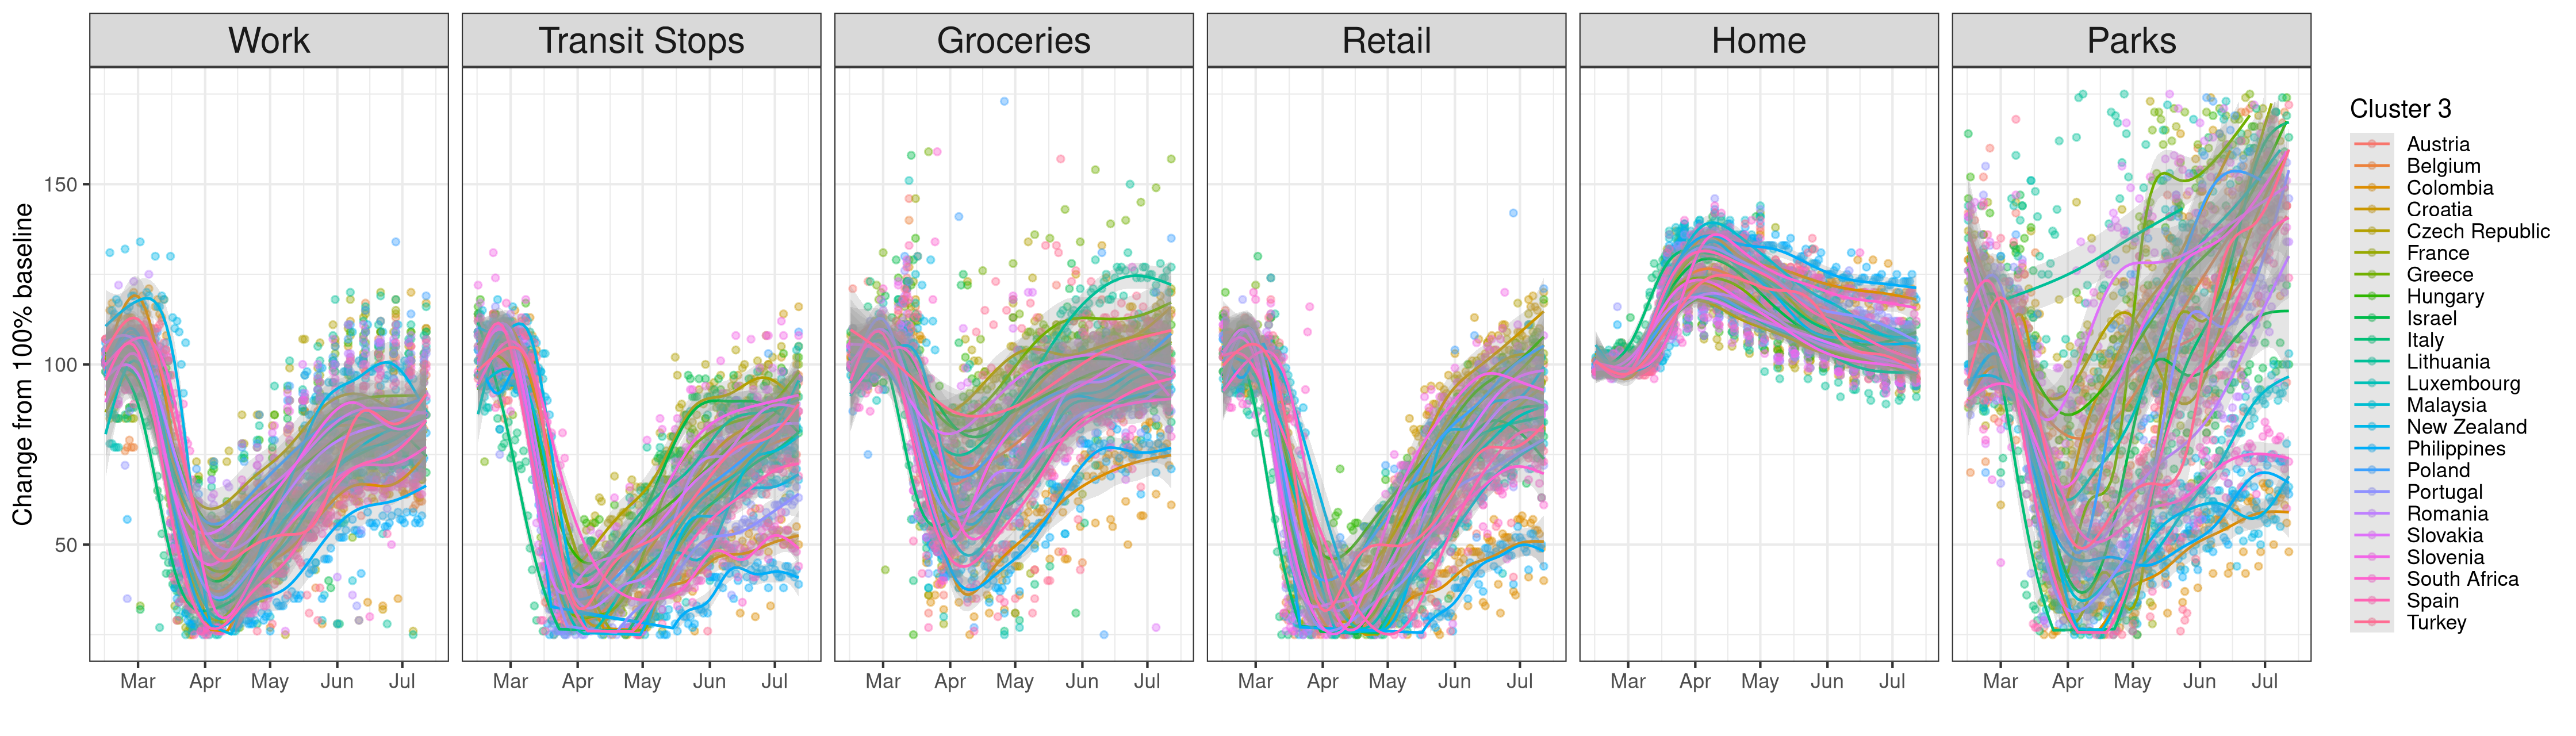
\includegraphics[width=\textwidth]{c3-activity}
  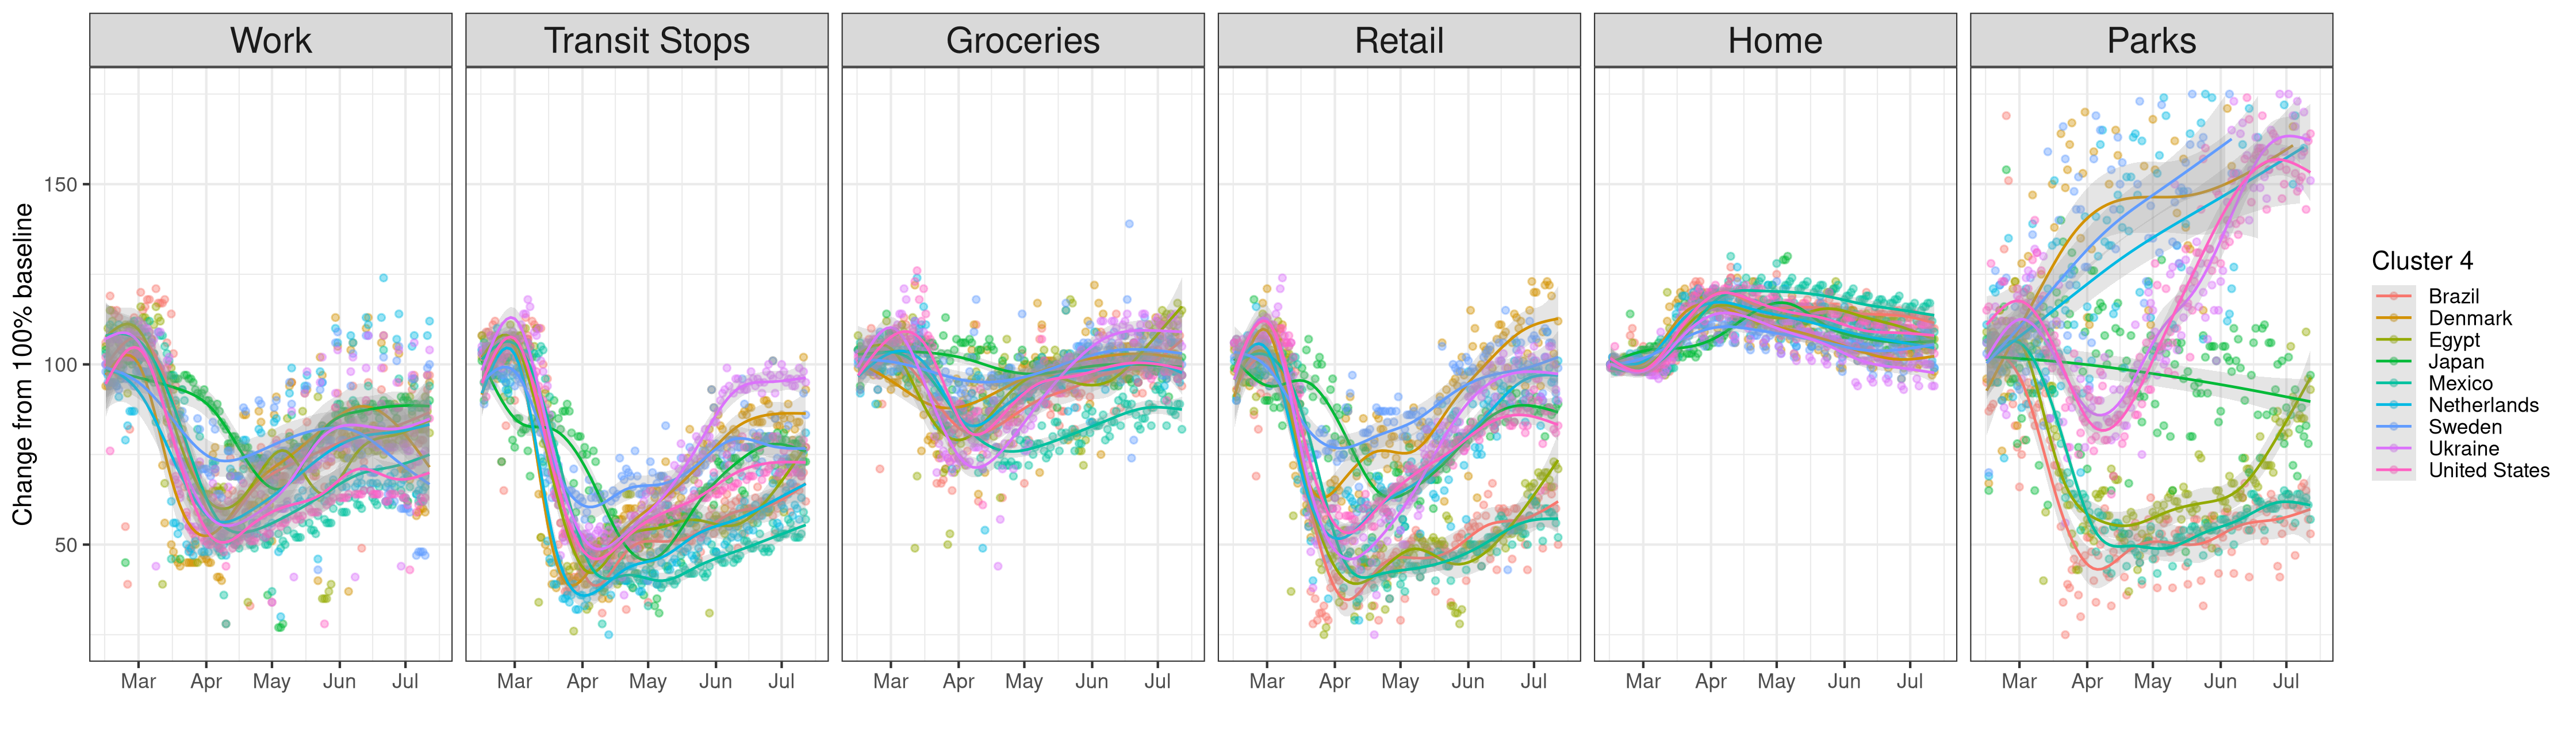
\includegraphics[width=\textwidth]{c4-activity}
  \caption{Activity changes from baseline (100\%) by cluster for Work ("work"), Transit stops ("tstop"), Grocery Shopping ("groc"), Retail and recreation ("reta"), Residence ("home") and Parks ("parks"). Trends are indicated using a generalized linear (GLM) fit for each country.}
  \label{fig:act}
\end{figure}


\subsection{Limitations}
No strictly or weakly exogenous variables are included in our model.
Further, there are other variables that can explain COVID-19 impacts not explicitly accounted for, particularly interventions.
These can be included as strictly exogenous variables in a future model.
Air passenger travel flows can also be incorporated as weights on weakly exogenous (foreign) variables.


\section{Conclusion and future work}

 
% \section{Author Contribution Statement}
% The authors confirm contribution to the paper as follows: \\
% Study conception and design: \\
% Analysis and interpretation of results: \\
% Manuscript preparation:

%\section{Acknowledgment}

\bibliography{references.bib}
\bibliographystyle{trb}


\end{document}

%%% Local Variables:
%%% mode: latex
%%% TeX-master: t
%%% End:

